\chapter{Introduction}
\label{chap:intro}

\section{Problem Statement}

Computing is ubiquitous, in science, engineering, business and
everyday life; and in cloud, desktop, and handheld.  Most of today's
programs run on multicore processors, and as a result they interact and
interfere.  It is important to control the
interaction and reduce the interference, for achieving not just
good performance, but also stable performance in a
dynamic environment; not just for parallel code, but also sequential
applications running in parallel.

Cache sharing is the primary cause of program interference.  Modern
applications spend most of the time accessing memory, and
most memory accesses, over 99\% typically, happen in cache.  On a
commodity system today --- 2 to 8
processors  (sockets), 2 to 6 physical cores per processor, and 2 to 4 hyperthreaded logical cores per physical core --- nearly a hundred programs
can run together in parallel.  

Partitioned cache solves the interference problem by program
isolation. However, cache partitioning is wasteful when only one program is
running and inefficient when co-run programs share data.  Current
multicore processors use a mix of private and shared cache. For
example, Intel Nehalem has 256K L2 cache per core and 4MB to 8MB L3
cache shared by all cores. IBM Power 7 has 8 cores, with 256KB L2
cache per core and 32MB L3 shared by all cores.

Depending on which CPU they are using, programs
interact in different ways.  Physical cores have private
cache at the first and second levels but share the last level cache.
Logical cores share the cache at all levels.  Different processors do
not share cache.  However, they share the memory bandwidth, and the
demand of memory bandwidth depends entirely on the performance of the
cache.  In addition, some caching policies, e.g. inclusive cache on
Intel machines, may induce indirect interaction, where a program may lose data in
its private cache due to the data access by another program in the shared
cache.

% eviction in the shared cache necessitates the eviction in the
% private  cache, 

The advent of cache sharing is reminiscent of the dawn of memory
sharing in early days of computing when time sharing was
invented.  The problem of memory management has been well studied
and solved, and modern operating systems manage memory for a large number of programs as a matter of course.
However, cache is managed by hardware not the operating system.

The problem of cache sharing is more complex.  Cache has multiple
levels and varying mixes of exclusivity and sharing.  Events of cache
accesses and replacements are orders of magnitude more frequent than memory
access and paging.  A single program may access cache a billion times
a second and can wipe out the entire content of the cache in less than
a millisecond.  The intensity multiplies when more programs are run
in parallel.  Furthermore, the size of cache is fixed on a given machine.
One cannot get online and buy more cache as one can with memory.

Cache interference is asymmetrical, non-linear, and circular.  The
asymmetry was shown in early experiments by \cite{Zhang+:EuroSys09} at
Rochester and confirmed by later studies.
In a pair-run experiment we conducted using Zhang's setup, one program
becomes 85\% slower, while its partner is only 15\% slower.  The
interference changes from program to program.  The effect depends not
as much on how many programs are running as on which programs are
running.  Finally, the interference has self feedback because the behavior of
one program affects the peer programs which affect itself.

\section{All-window Footprint}

Locality is a basic property of a computing system.  \cite{Denning:TSE80}
defined locality as ``a concept that a program favors a subset of its
segments during extended intervals (phases).'' 
There is a difference between the data that a program has
and the data that the program is actively using.  The latter is a
subset of the former.  \cite{Denning:CACM68} coined the widely used term \emph{the working set}
to refer to the active data subset.

The performance depends on how fast a computer system
provides access to the active data subset.  The access time of 
the other data is irrelevant.  
Locality analysis, as it
quantifies the active data usage, is naturally a pre-requisite to
memory system design, for the oft quoted reason``we cannot improve
what we cannot measure.''

This dissertation measures the active data usage by a concept we call
the \emph{footprint}.  A footprint is the amount of data accessed in a
time window.  It is the size of the active data.  

As an illustration, let's use the
word ``footprint'' as a short trace and treat its 9 occurrences of 7 letters
as 9 accesses to 7 data blocks.  Every sub-string is a time window in the trace.  Its footprint is the number of
distinct letters in the sub-string.  

\begin{figure}[h]
\centering
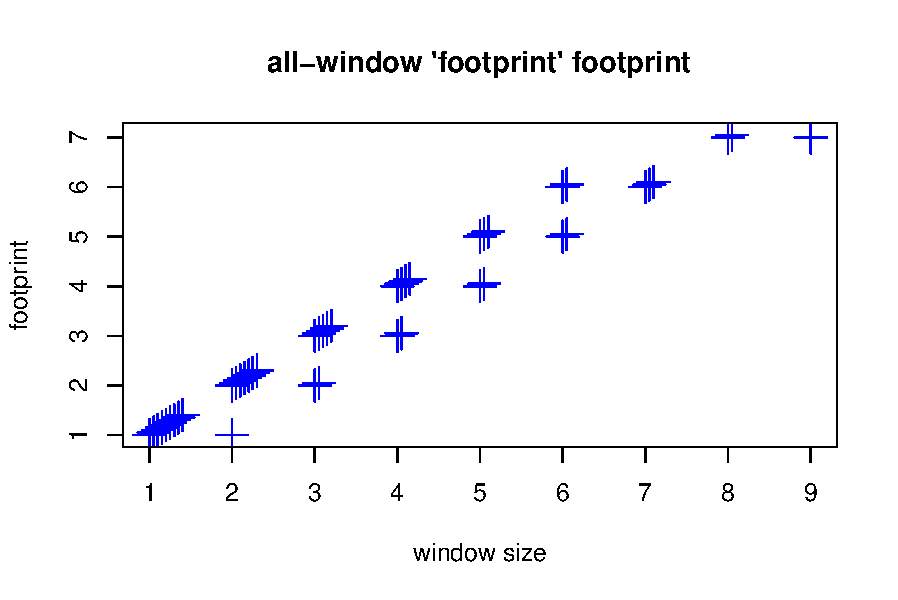
\includegraphics[width=14cm]{figures/intro/footprintfp}
\caption{The footprint of 36 windows in the contrived 9-element trace ``footprint''}
\label{fig:fpfp}
\end{figure}

There are 45 windows in the 9-element trace (9 choose 2 plus 9).  The 45 footprints are
plotted in Figure~\ref{fig:fpfp}.  As the window size (x-axis) increases from
1 to 9, and the footprint (y-axis) grows from 1 to 7.  Take for example the extreme cases.  The shortest
windows have a unit length.  There are 9 such windows, and their
footprint is obviously 1.  The longest
window is the whole trace, and the footprint is 7.  

It is natural that a longer period of execution accesses 
a greater amount of data.  The footprint quantifies the relation by showing the size of active data in all periods of
execution, as shown in the plot in Figure~\ref{fig:fpfp} for
the example trace.  

In practice, the footprint is too numerous to enumerate.  The
number of time windows is quadratic to the length of the
trace.\footnote{If the trace length is $n$, the number of windows (and
  hence footprints) is ${{n}\choose{2}} + n = \frac{n*(n+1)}{2}$ or $O(n^2)$ asymptotically.}
Assuming a program running for 10
seconds on a 3GHz processor, we have $3E10$ CPU cycles in
the execution and $4.5E20$
distinct windows.  

\begin{figure}[]
  \centering
  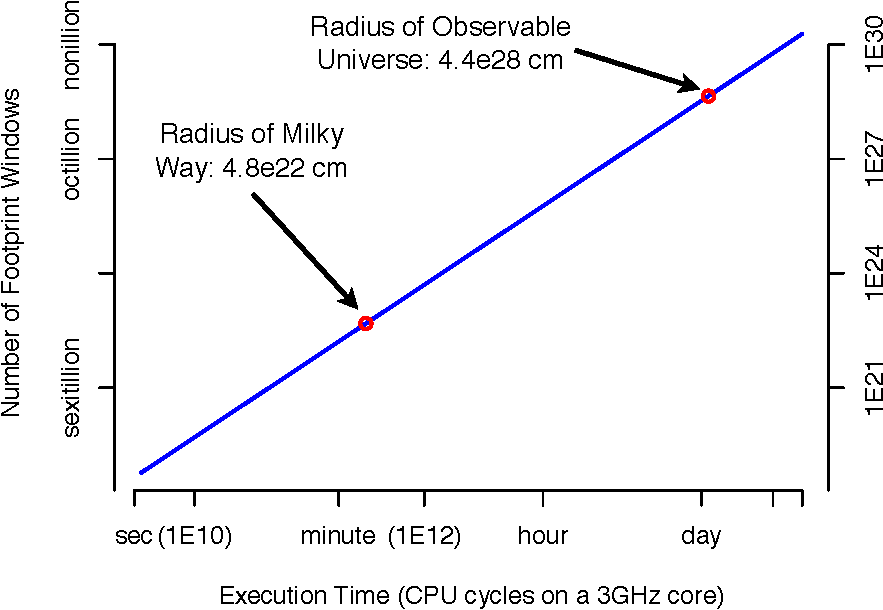
\includegraphics[width=11cm,height=8cm]{figures/intro/WindowSizes2}
  \caption{The scale of the problem shown by the number of footprint
    windows in a program execution, compared to the size of a galaxy and the universe.  Reproduced from \cite{Brock+:BDAW13}.}
  \label{fig:bigdata}
\end{figure}

\cite{Brock+:BDAW13} described program analysis as a Big Data problem, 
and showed the scale of the problem by the number of time
windows in an execution.
Figure~\ref{fig:bigdata} shows that as the length of execution increases from 1
second to 1 month, the number of CPU cycles ($n$) ranges from $3E9$ to
$2E15$, and the number of distinct execution windows $n \choose 2$
from $4.5E18$ to $5.8E29$, that is, from 4 sextillion to over a half
nonillion.  

As a dynamic analysis problem, the scale 
quickly reaches the size of any static problem.  As a comparison, 
the figure shows the radius of the Milky Way in centimeters, 48 sextillion,
and the radius of the observable universe, 44 octillion.

The purpose of a footprint theory is to overcome the enormity of the
analysis problem, characterize the active data usage in all windows
and make it useful for system analysis and optimization.

\begin{comment}
``footprint''

% Ruby script for generating (x,y) coordinates for the footprint plot

afp = {}
afp[1] = [1,1,1,1,1,1,1,1,1]
afp[2] = [2,1,2,2,2,2,2,2]
afp[3] = [2,2,3,3,3,3,3]
afp[4] = [3,3,4,4,4,4]
afp[5] = [4,4,5,5,5]
afp[6] = [5,5,6,6]
afp[7] = [6,6,6]
afp[8] = [7,7]
afp[9] = [7]

# frequency count
freqs = Hash.new{ 0 }

def perturb( wfp, freqs, delta = 0.05 ) 
  freq = freqs[wfp]
  freqs[wfp] = freq + 1
  wfp.collect{ |i| i + freq*delta }
end

xs, ys = [], []
afp.each do |ws, fps|
  fps.each do |fp| 
     x, y = perturb([ws,fp], freqs)
     xs << x.to_s
     ys << y.to_s
  end
end
puts "x = c( #{xs * ', '} )\ny = c( #{ys * ', '} )"

% R script for plotting, pch=3 is +, 4 is cross, see http://sphaerula.com/legacy/R/plotSymbols.html

dev.new(width=6, height=4)
plot( x, y, pch=3, cex=2, col="blue", xlab = "window size", ylab = "footprint", main = "all-window 'footprint' footprint" )
axis(1, seq(9), seq(9))
dev.copy2pdf(file="footprintfp.pdf")
dev.off()

\end{comment}

\section{A New Locality Theory}
\label{sec:intro:theory}

For locality analysis, the basic unit of information is a data access,
and the basic relation is a data reuse.  The theory of locality is
concerned with the fundamental properties of data accesses and reuses,
just as the graph theory is with nodes and their links.

The core of the dissertation is a new locality theory consisting of a
set of formal definitions, algorithms and properties based on the
concept of the footprint.  This section introduces the four components of the theory and their supporting techniques.

\paragraph{Footprint Measurement}
The enormous scale of all-window analysis is tackled by a series of
three algorithms.  Each is two orders of magnitude more efficient than
the previous one.

\begin{itemize}
\item \emph{Footprint distribution analysis}, which enumerates 
  all $O(n^2)$ footprints in $O(n \log m)$ time, where $n$ is the 
  length of the trace and $m$ the maximal footprint.
\item \emph{Average footprint analysis}, which reduces the cost to
  linear time $O(n)$ by computing the average without enumerating all
  footprints.
\item \emph{Footprint sampling}, which samples limited-size windows and reduces the cost to sub-linear.
\end{itemize}

The distribution analysis is the first algorithm to measure
all-window footprint.  As it actually enumerates all footprints, it
finds the largest, smallest, median, average, and any percentile
footprint for each window length.  However, the cost is sometimes
thousands of times slowdown.

The second algorithm computes just the average footprint, and the
cost is reduced from a thousand times slowdown to about 20 times.  Being a linear time
algorithm, it is scalable in that the cost increases proportionally to
the length of the program execution.

The cache on a real machine has a finite size, so an analysis does
not have to consider windows whose footprint is greater than the cache
size.  In addition, the behavior of a long running
program tends to repeat itself.  Furthermore, on modern
processors, the analysis can be carried out on a separate core in
parallel with the analyzed execution.
Footprint sampling specializes and parallelizes the
analysis for a specific machine and program.  The average
cost is reduced to 0.5\% of the running time of the unmodified execution.

The algorithmic development attains immense gains in both
computational complexity and implementation efficiency.  As the baseline, the first algorithm is
already a breakthrough since there was no previous viable solution for
all-window analysis.  The second and the third algorithm each
improves efficiency by another
orders of magnitude, eventually making it fast enough for
real-time analysis.  This has a beneficial impact elsewhere, because
the footprint can be used to compute other locality
metrics, as we will see in the next part of the footprint theory.

\paragraph{Composability}
As a locality metric, footprint is unique because it is composable.  
Let the average footprint of a program be $prog.fp(x)$ for window
length $x$.  If we have $k$ programs $prog_1, prog_2, \dots,
prog_k$ actively sharing the cache, the aggregate footprint is
the sum of the individual footprints.

$$ corun.fp(x) = \sum_{i=1}^k prog_i.fp(x) $$

In comparison, the miss ratio is not composable.  Consider two
programs sharing the cache.  The co-run miss ratio will change
compared to the solo-run miss ratio since each program has
now a fraction instead of the whole cache.  The change in miss ratio, as mentioned
earlier, is asymmetrical, non-linear and affected by circular
feedback.  As a result, we cannot directly add the solo-run miss ratio 
to compute the co-run miss
ratio, as we can with the footprint. 

Another locality metric is reuse distance.  Reuse distance does
not depend on cache parameters but as we will explain
in Section~\ref{sec:back:rd}, it is also not composable.

% two bodies of water can be composed into a bigger body but two bags
% cannot be composed into a bigger bag.

As mentioned earlier, we can measure the average as well as
the distribution of footprints.  
The average footprint is immediately composable.  The distribution, although composable, requires
a convolution which is expensive to compute and difficult
to visualize.  In this thesis except in Section~\ref{sec:all-fp}, 
the term footprint when unqualified means the average
footprint.

The next question is whether the composability from the footprint 
can help in analyzing the miss ratio and other locality metrics in
shared cache.  This is solved in
the third part of the new theory.

\paragraph{Locality Metrics Conversion}
The footprint is convertible with a number of other metrics,
as we will show in Chapter~\ref{chap:model}.  For example, let $mr(c)$ be the miss ratio
for cache size $c$.  The conversion formula we will derive is the
following:

$$\textit{mr}(c) = \frac{\textit{fp}(x+\Delta x) - fp(x)}{\Delta x}$$

\noindent where $c = \textit{fp}(x)$.  If these are continuous
functions, we would say that the miss ratio is the derivative function
of the footprint.  

The higher order mathematics implies stricter
properties.  The derived metric, the miss ratio, should be
non-decreasing.  For this to hold in all cases, the source function 
must be not just non-decreasing but also
concave.  We will prove that the average
footprint has this stronger property.  

The conversion is reversible.  If we have the miss ratios of all cache
sizes, we can reverse the formula and compute the average
footprint.  The reverse process is the analogous of integration for
a discrete function.  

% Let the inter-miss time for cache size $k$ be $im(k) =
% \frac{1}{mr(k)}$, the reciprocal of the miss rate.  The window length
% of footprint of size $c$

Combining footprint composition and metrics conversion, we can see immediately that if 
we treat co-run programs as one composite task, the
co-run miss ratio can be computed from the aggregate footprint.
Figure~\ref{fig:conversion} shows the derivation by adding
the individual footprints and then converting the sum to the miss ratio.  

\begin{figure}[h]
\centering
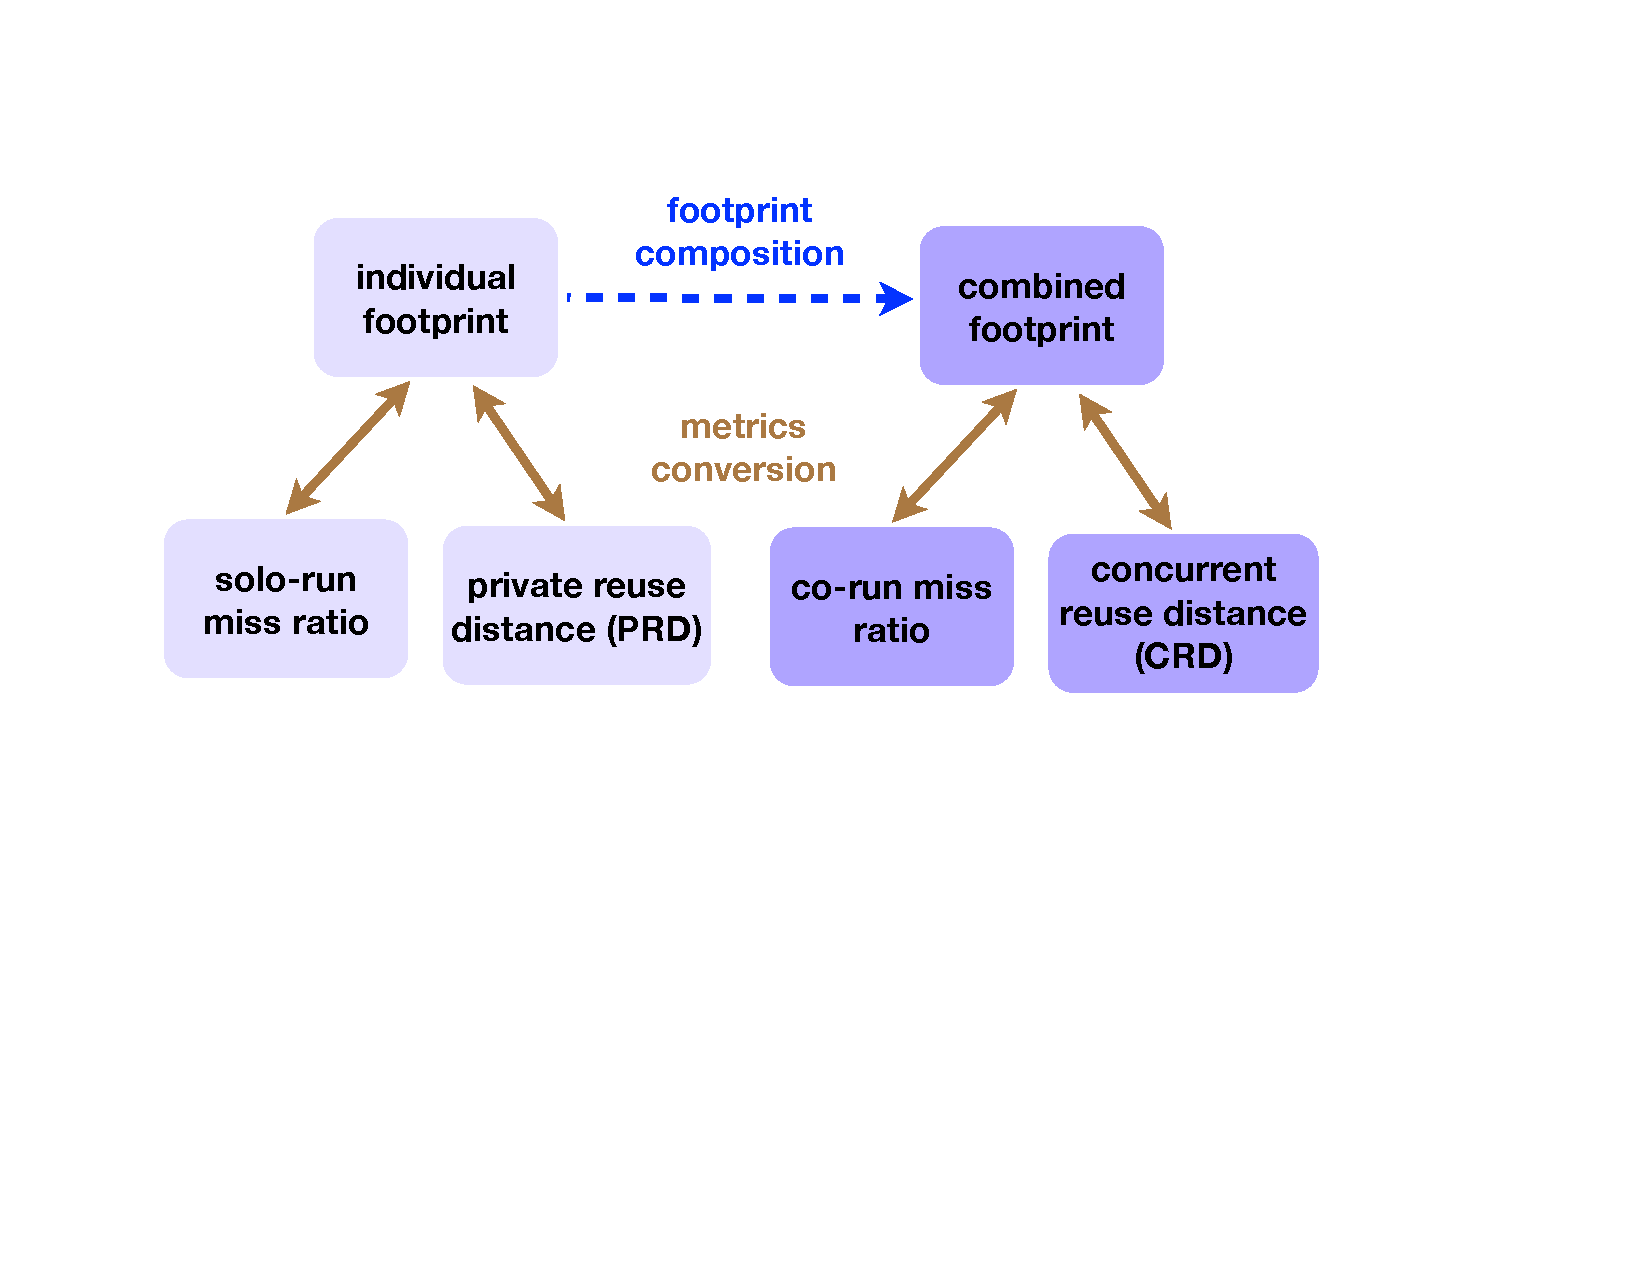
\includegraphics[width=10cm]{figures/intro/conversion}
\caption{The joint use of two theoretical properties: composition (dotted line) and conversion (solid lines)}.
\label{fig:conversion}
\end{figure}

Since the conversion formula is reversible, we can switch 
between the footprint and the miss ratio and compose the latter indirectly through the former.  
First, we compute the individual
footprint from the individual miss ratios (of all cache sizes).  Then 
we 
add the individual footprints and finally compute the co-run miss
ratio in the shared cache (of all sizes).  Figure~\ref{fig:conversion}
shows this type of deduction and others that are made possible by
composition and conversion.  In particular, the figure shows how to compose another locality
metric, the reuse distance.  We use the terms private reuse distance (PRD)
and concurrent reuse distance (CRD), as introduced by \cite{WuY:PACT11,Wu+:ISCA13}.

The solution of composition raises the problem of decomposition.
The co-run miss ratio does not tell us the contribution from each
program.  To see the individual effects, we need more elaborate models.

\paragraph{Composable Locality Models}
We say a model is composable if the co-run result can be computed from
solo-run results, not just for the co-run group as a whole but also
for the co-run effect on each individual program.  In other words,
a composable model must be both composable and decomposable.

First, let's summarize the three reasons that footprint-based models
are general and efficient for composition.  The footprint is

\begin{itemize}
\item \emph{Machine independent.}  The analysis is based on data
  accesses, not cache misses.  It takes a single pass to analyze a
  trace for all cache sizes, and the result is not affected by program
  instrumentation.  In comparison, it is inescapable for direct measurement to be
  affected by instrumentation.
\item \emph{Clean-room statistics.}  The
  footprint of one program can be measured in a co-run environment, unperturbed by
  other programs.  The clean-room effect solves the chicken-or-egg
  problem of direct measurement: the behavior of one program depends on 
  its peer, but the peer behavior in turn depends on itself.
\item \emph{Peer independent.}  Locality metrics are
  defined on and for a program itself, independent of co-run peers.
  The analysis of cache sharing does not require actual cache 
  sharing.  The co-run effect is computed rather than measured.
\item \emph{Static composition.}  There are $2^P$ co-run combinations
  for $P$ programs.  The footprint model can predict the interference
  in these $2^P$ runs by testing $P$ single-program runs.  For the $P$
  sequential runs, one can choose to run them one by one or some of
  them in parallel to increase speed. The composition is static if
  there is no actual co-run; otherwise we say the composition is
  dynamic.  Here dynamic composition means parallel testing.  Static
  composition does not need parallel testing at all.
\end{itemize}

To compute the co-run effect on each individual program, the
dissertation describes three models.  The models solve the decomposition
problem as a composition problem: how one program is affected
by its peers.

% formalism must work out so the sum of the predicted individual
% effects gives the same result as the predicted overall effect.

\begin{itemize}
\item \emph{Composition by reuse distance and footprint} 
Variations of this model were invented by
  \cite{ThiebautS:TOCS87} and \cite{Suh+:ICS01} for time-sharing systems (time-switched cache sharing) and \cite{Chandra+:HPCA05} for multicore (continuous cache sharing).  With fast
  footprint measurement, we will show that the cost of the model is limited by the time
  required for reuse distance measurement.
\item \emph{Composition by footprint only} The second model converts the
  footprint into reuse distance, so it no longer needs to measure 
the reuse distance and can be
  hundreds of times faster.
\item \emph{Composition by program pressure and sensitivity} The last
  model is as fast as the second model but more intuitive and easier
  to use.  It characterizes the behavior of a program
  by two factors, pressure and sensitivity.  The two can be
  visualized as two curves.  Performance composition is as simple as
  looking up related values on the two curves.
\end{itemize}

Using the composable models, the thesis will answer a number of
long-standing questions about shared cache, including:

\begin{itemize}
\item Is there a machine independent way to compare programs by their
  shared cache behavior?  How do programs differ within and
  between application domains?
\item How does the interference correlate with the miss ratio?  If a
  program has a higher miss ratio, does it always exert a higher interference?
\item Can the shared cache be viewed as a confederation of per-program
  partitions?  In the shared cache, the division of space is dynamic and
  demand driven.  Does the dynamism provides an inherent advantage
  for cache sharing over cache partitioning?
\end{itemize}

These models are theoretical.  They are appealing due to the
generality.  The footprint is defined on a program trace without
knowing co-run peers or machine parameters (other than having shared
cache).  There are many sources of error due to the fact that the
basic models do not consider the effect of cache associativity,
program phase behavior, the time dilation due to interference, the
filtering effect in a multi-level cache hierarchy, and the impact of
the prefetcher.  A theory must be validated to be practically
relevant.  The thesis will show evaluate these model on real systems
and compare theoretical predictions with actual miss counts measured
by hardware counters.  It will also show extensions of the models to
consider time dilation, cache associativity, and program phases.
 
By developing and validating the new theory, this thesis will
quantify the essential aspects of program behavior in shared cache and
as a result enhance our ability to understand and manage program
interaction on multicore systems.


\section{Thesis Statement and Organization}

{\bf Thesis statement}  
\emph{The interaction of computer programs in shared cache can be
efficiently and accurately modeled and dynamically optimized using 
a footprint theory of locality that includes footprint measurement,
conversion, and composable modeling.}

The technical content is organized in five chapters as follows. 

\begin{itemize}
\item Chapter~\ref{chap:background} gives the background of locality
theories and techniques, including locality metrics and measurements
and previous cache sharing models. 

\item Chapter~\ref{chap:fp} presents the three algorithms for
  footprint measurement.  The first measures the footprint
  distribution, the second the average footprint.  The first two
  algorithms are precise and asymptotically efficient.  The third
  algorithm improves the practical efficiency through footprint
  sampling.

\item Chapter~\ref{chap:model} presents a higher order theory for the
  mutual conversion between five locality metrics.  It shows
  the correctness condition for the conversions.  Theoretically, it extends
  the work-set theory and confirms Denning's Law of Locality.
  Empirically, it enables near real-time locality analysis.

\item Chapter~\ref{chap:corun} describes the pressure-sensitivity
  model where the behavior of a program in shared cache is completely
  characterized by just two factors.  The model is built from the new
  theory, the calculation (of miss ratios) extremely simple, and the
  result consistently accurate.

\item Chapter~\ref{chap:regroup} presents a cache-conscious task
  regrouping framework, which uses the new models to minimize cache
  interference on multicore processors. 
\end{itemize}

The style of the work is mixed, so is the presentation: formal and
algorithmic for footprint measurement, mathematical for metrics
conversion, and experimental and scientific for performance
calibration and validation.

